\documentclass{article}
\usepackage[utf8]{inputenc}
\usepackage{amsmath}
\usepackage{ dsfont }
\usepackage{graphicx}
\usepackage{array}


\title{Trabajo práctico de R}
\author{Kevin Frachtenberg, Ruslan Sanmartin Sobol , Celeste Rodriguez}
\date{27 Junio 2017}

\begin{document}

\maketitle

\section{Ejercicio 1}

$X_1,...,X_n =$ m.a. iid U[0,b]

1) $b_{mom}$: $\frac{\sum_{i=1}^{n} X_i}{n} = \mathbb{E}[X] = \frac{b}{2}$. $\Longleftrightarrow X_n = \frac{b}{2} \Longleftrightarrow b_{mom} = 2X_n$
\newline

2) $b_{mv}$: L(b) $= \prod_{i=1}^{n} \frac{1}{b-0} \mathds{I}_{[0,b]}(x_i)$


\[
L(b) = 
     \begin{cases}
       \text{$\prod_{i=1}^{n}$ $\frac{1}{b}$} &\quad\text{si max($x_i$) $\leq$ b}\\
       \text{0} &\quad\text{si no}\\ 
     \end{cases}
=
     \begin{cases}
       \text{$(\frac{1}{b})^n$} &\quad\text{si max($x_i$) $\leq$ b}\\
       \text{0} &\quad\text{si no}\\ 
     \end{cases}
\]

Vemos que L(b) es decreciente si b mayor o igual que el máximo de los $x_i$ y es constantemente 0 en caso contrario. Por lo tanto, encontramos que $b_{mv} = max(x_i)$

\newline

\section{Ejercicio 3} $b_{mom} = 0.8357194$, $b_{mv} = 0.958102$, $b_{med} = 0.6800235$. Los errores respectivamente son $0.1642806$, $0.04189796$, $0.3199765$

\section{Ejercicio 6}
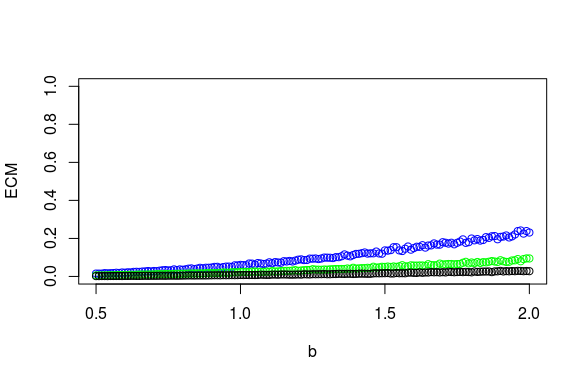
\includegraphics[scale=0.85]{ej6.png}
En este gráfico, los puntos azules representan el estimador de mediana, mientras que los verdes al de momentos y los negros al de máxima verosimilitud. Observamos que cuando b es chico, los tres estimadores se comportan de manera similar. Sin embargo, a medida que aumenta b, el ECM del $b_{med}$ es el que más aumenta. Creemos que como el rango de valores que puede tomar la distribución es mayor (uniforme entre 0 y b) y $b_{med}$ depende de la mediana de la muestra, es menos probable que $b_{med}$ esté cerca de b. Por otro lado, el ECM de $b_{mom}$ también aumenta conforme aumenta b (aunque en comparación a $b_{med}$ en menor medida) mientras que $b_{mv}$ se mantiene prácticamente constante (siempre cerca de 0). Finalmente, elegimos $b_{mv}$ como estimador.
\section{Ejercicio 7}
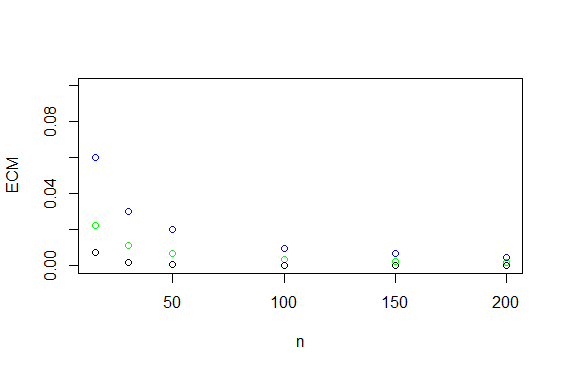
\includegraphics[scale=0.85]{ej7.png}
En este segundo gráfico, cada color representa al mismo estimador que en el Ejercicio 6. El estimador con menor ECM es $b_{mv}$, luego le sigue $b_{mom}$ y por último $b_{med}$. En los tres casos a medida que aumenta el tamaño de la muestra, menor es el ECM.  Se puede ver como para una muestra grande (n=200) los tres estimadores se comportan de manera similar. Estas observaciones nos permiten sospechar que los tres estimadores son consistentes, a medida que se aumenta el tamaño de la muestra el sesgo decrece (la esperanza del estimador se parece cada vez más a b) y la varianza también (el comportamiento de los tres se hace más parecido conforme aumenta n). Sin embargo, cuando la muestra es chica (n<50) $b_{med}$ se aleja mucho más de b que el resto de los estimadores. Cuando n es chico, $b_{mv}$ es el de menor ECM por lo que lo elegimos como estimador.

\section{Ejercicio 8}
bmom= 3.642933
Bmv= 20.1
Bmed= 1.06
Observamos que el $b_{med}$ es el que se acerca más al valor real de b (que es 1). Esto se debe a que $b_{med}$ es resistente a valores atípicos (ya que depende de la mediana por lo que no será afectado por un solo outlier). En nuestra muestra, hay un valor que está muy lejos del resto (20,1) y este hace que $b_{mom}$ y $b_{mv}$ se vean muy afectados. Por eso, en ciertos casos cuando se presentan estos valores atípicos es conveniente estimar mediante un $b_{med}$. 


\newpage

\section{Ejercicio 9}
\newline

\begin{table}[h!]
\centering
\caption{Tabla comparativa}
\label{my-label}
\begin{tabular}{llll}
\hline
\multicolumn{1}{|l|}{}                  & \multicolumn{1}{l|}{\textbf{MOM}} & \multicolumn{1}{l|}{\textbf{MV}} & \multicolumn{1}{l|}{\textbf{MED}} \\ \hline
\multicolumn{1}{|l|}{\textbf{Sesgo}}    & \multicolumn{1}{l|}{0.3905915}   & \multicolumn{1}{l|}{2.823237}   & \multicolumn{1}{l|}{0.005074287}    \\ \hline
\multicolumn{1}{|l|}{\textbf{Varianza}} & \multicolumn{1}{l|}{3.441915}     & \multicolumn{1}{l|}{190.2666}    & \multicolumn{1}{l|}{0.0616792}   \\ \hline
\multicolumn{1}{|l|}{\textbf{ECM}}      & \multicolumn{1}{l|}{3.594477}     & \multicolumn{1}{l|}{198.2373}    & \multicolumn{1}{l|}{0.06170494}    \\ \hline

\end{tabular}
\end{table}
Observamos que tanto el $b_{mom}$ como el $b_{mv}$ ambos tienen un sesgo distinto a 0, mientras que el sesgo de $b_{med}$ es prácticamente 0 (es decir el valor esperado de $b_{med}$ es b). Además, el estimador de momentos y el de máxima verosimilitud presentan varianza y ECM mucho mayor que el de $b_{med}$ (sobre todo el $b_{mv}$). Esto se debe a que el valor que está alejado del resto de los valores de la muestra (el primer elemento es cien veces más grande) hace que crezca tanto la varianza como el ECM de los primeros dos estimadores mientras que por la naturaleza del $b_{med}$ (mira el valor intermedio de la muestra), este estimador no es afectado tanto por el outlier. Elegimos el $b_{med}$ ya que no solo tiene el menor sesgo, sino también al ser resistente a valores atípicos, tiene menor ECM y varianza por lo que es más preciso y se acerca más al valor real de b.

\end{document}
